\section{Experiments}\label{sec:experiments}
To evaluate the performance of our approach,  we implemented
a prototype system in Java, following a traditional iterator model.
For our experiments we plan and execute queries
for two separate survey-based data sets, showing that our system
is ideal for early dataset exploration.

\subsection{Data sets} \label{subsec:datasets}
\subsubsection{Center for Disease Control: Surveys}
For our first set of experiments, we use survey data collected by the 
Center for Disease Control and Prevention (CDC) in the United States. In particular, we
experiment on a set of tables collected as part of the National
Health and Nutrition Examination Survey (NHANES), a series of studies
conducted by the CDC on a national sample of several thousand individuals\cite{cdc-data}.
The data consists on survey responses, physical examinations, and laboratory
results, amongst others. Our dataset corresponds to the 2013-2014 NHANES
and is available for direct download on the CDC's organization site on 
kaggle.com, a popular data science website.

There are a total of 6 tables associated with the NHANES data set. For purposes
of our experiments, we use three tables:

\begin{itemize}
	\item Demographics: outlines demographic information of subjects
	\item Examinations: physical exam results
	\item Laboratory: laboratory exam results
\end{itemize}

The original tables have a large number of attributes, in some cases providing more granular
tests results or alternative metrics. In order to simplify the presentation and
exploration of queries, we focused on a subset of the attributes for each table.
Table~\ref{table:nhanes-description} shows the attributes selected, along with the
percentage of nulls. It is worth noting that for readability, we have replaced the
NHANES variable names with self-explanatory attribute names.

\begin{table}
    \centering
    \begin{subtable}{0.5\textwidth}
        \centering
       \begin{tabular}{llr}
\toprule
\textbf{Attribute} &  \textbf{\% Missing} \\
\midrule
age\_months &      93.39 \\
age\_yrs &       0.00 \\
gender &       0.00 \\
id &       0.00 \\
income &       1.31 \\
is\_citizen &       0.04 \\
marital\_status &      43.30 \\
num\_people\_household &       0.00 \\
time\_in\_us &      81.25 \\
years\_edu\_children &      72.45 \\
\bottomrule
\end{tabular}

        \caption{Demographics}
    \end{subtable}
    \begin{subtable}{0.5\textwidth}
        \centering
        \begin{tabular}{lS[table-format=2.2]}
\toprule
\textbf{Attribute} &  \textbf{Missing} \\
\midrule
albumin &      17.95\ \% \\
blood\_lead &      46.86\ \% \\
blood\_selenium &      46.86\ \% \\
cholesterol &      22.31\ \% \\
creatine &      72.59\ \% \\
hematocrit &      12.93\ \% \\
id &       0.00\ \% \\
triglyceride &      67.94\ \% \\
vitamin\_b12 &      45.83\ \% \\
white\_blood\_cell\_ct &      12.93\ \% \\
\bottomrule
\end{tabular}

%%% Local Variables:
%%% mode: latex
%%% TeX-master: "../main"
%%% End:

        \caption{Laboratory Results}
    \end{subtable}
       \begin{subtable}{0.5\textwidth}
        \centering
        \begin{tabular}{llr}
\toprule
 Table &                Attribute &  \% Missing \\
\midrule
 exams &        arm\_circumference &       5.22 \\
 exams &      blood\_pressure\_secs &       3.11 \\
 exams &  blood\_pressure\_systolic &      26.91 \\
 exams &          body\_mass\_index &       7.72 \\
 exams &                cuff\_size &      23.14 \\
 exams &       head\_circumference &      97.67 \\
 exams &                   height &       7.60 \\
 exams &                       id &       0.00 \\
 exams &      waist\_circumference &      11.74 \\
 exams &                   weight &       0.92 \\
\bottomrule
\end{tabular}

        \caption{Physical Results}
    \end{subtable}
    \caption{Missing values in CDC NHANES 2013-2014 data}
    \label{table:nhanes-description} 
\end{table}

All tables used consists of 10 attributes. The laboratory and examinations data,
referred to as \textit{labs} and \textit{exams} in our queries, consist of 9813 rows,
while the demographics data (\textit{demo}) have 10175 rows.

\subsubsection{freeCodeCamp: 2016 New Coder Survey}
For our second set of experiments, we chose to use data collected
by freeCodeCamp as a part of a survey of new software developers
(both professional and amateur)\cite{fcc-data}. freeCodeCamp is an open-source
community that intends to help users learn how to program. In addition,
to providing training material for users, it also pairs users with
nonprofits to develop software solutions. Their \textit{2016 New Coder Survey} consists of responses by over 15,000 people to 48 different
questions. The survey targeted users who were in one way or another
related to coding organizations.

For our purposes, we use a version of the data that has been 
pre-processed, but where plenty of missing values remain. It is
worth noting that given the table design (where many attributes
are related), many of these missing values are to be
expected. The dataset we started with had 15,620 rows and 113
columns. We chose 17 attributes, which are outlined in Table~\ref{table:fcc-description}, along with the percentage of missing values.

\begin{table}
   \centering
    \begin{tabular}{lr}
\toprule
            \textbf{Attribute} &  \textbf{\% Missing} \\
\midrule
age &      12.85 \\
attendedbootcamp &       1.54 \\
 bootcampfinish &      94.03 \\
 bootcampfulljobafter &      95.93 \\
 bootcamploanyesno &      94.02 \\
 bootcamppostsalary &      97.89 \\
childrennumber &      83.65 \\
citypopulation &      12.74 \\
commutetime &      46.61 \\
countrycitizen &      12.59 \\
gender &      12.00 \\
hourslearning &       4.34 \\
income &      53.08 \\
moneyforlearning &       6.02 \\
monthsprogramming &       3.88 \\
schooldegree &      12.43 \\
studentdebtowe &      77.50 \\
\bottomrule
\end{tabular}

    \caption{Missing values in FCC Survey Data}
   \label{table:fcc-description} 
\end{table}

For our final experiment, we introduce a simple aggregate query over data from the American Community Survey (ACS), which
provides a number of public data sets collected by the U.S. Census Bureau.
We used a cleaned version of the 2012 Public Use Microdata Sample (PUMS) data kindly provided by the authors of~\cite{akande2015empirical}.
Given that the data had been cleaned, we uniformly introduced missing values across 40 percent of the values. The final dataset consists
of 671,153 rows and 37 integer columns.

\subsection{Queries}
We collect a set of queries (Table~\ref{fig:queries}) that we think are both representative, in that they could reasonably be written by a user in the course of data analysis, and interesting to plan.

The queries on the CDC NHANES data consist not only of projections and selections,
but also interesting joins and aggregates. Our aim was to craft meaningful queries
that would provide performance figures relevant to practitioners who may use
similar datasets.

Queries 1-5 are on the CDC data. In Query~\ref{q1}, we calculate the average height for users based on their income data. In Query~\ref{q2},
we compare cholesterol levels for individuals at either tail of the income
spectrum and above a certain weight. In Query~\ref{q3},
we extract the maximum blood lead levels for children under the age of 6 years. In Query ~\ref{q4}, we calculate the average systolic blood pressure, by gender, for subjects with a body mass index indicating obesity. In Query ~\ref{q5}, we extract the age (in months), creatine level, and head circumference, for subjects with high creatine levels.

% Perhaps more school makes your head bigger :)

Queries 6-10 are on the FCC data. In Query~\ref{q6}, we calculate the average income for survey participants,
based on their bootcamp attendance. In Query~\ref{q7} estimates the average
age of women from the United States who participated. In Query~\ref{q8}, we 
calculate the average amount of money survey participants with student debt destined to
learning based on their school degree. In Query~\ref{q9}, we join the FCC data with a reference table provided
by the World Bank which summarizes GDP per Capita across various
countries\cite{worldbank-data}. The query calculates the average GDP-per-capita for participants based on whether or not they
attended a bootcamp. Finally, in Query ~\ref{q10}, we identify individuals from countries with GDP per-capita of \$5000 or
less who earn \$100,000 or more post-bootcamp.

Note that for all queries we have enumerated strings and encoded them with
an appropriate integer value.

\begin{table*}
\centering
 \begin{subtable}{\linewidth}
  \newcounter{queryno}
\begin{tabular}{cl}
\toprule
\# & \multicolumn{1}{c}{Query} \\
\midrule
1 & 
\begin{minipage}{6in}
\begin{lstlisting}[breaklines]
SELECT income, AVG(height)
FROM demo, exams
WHERE demo.id = exams.id
GROUP BY income;
\end{lstlisting}
\end{minipage}\refstepcounter{queryno} \label{q1} \\
2 & 
\begin{minipage}{6in}
\begin{lstlisting}[breaklines]
SELECT income, AVG(cholesterol)
FROM demo, exams, labs
WHERE demo.id = exams.id AND exams.id = labs.id AND
      income >= 13 AND income <= 15 AND weight >= 63
GROUP BY income;
\end{lstlisting}
\end{minipage}
\refstepcounter{queryno} \label{q2} \\
3 & 
\begin{minipage}{6in}
\begin{lstlisting}[breaklines]
SELECT MAX(blood_lead)
FROM demo, exams, labs
WHERE demo.id = labs.id AND labs.id = exams.id AND age_yrs <= 6;
\end{lstlisting}
\end{minipage}\refstepcounter{queryno} \label{q3}\\
4 & 
\begin{minipage}{6in}
\begin{lstlisting}[breaklines]
SELECT gender, AVG(blood_pressure_systolic)
FROM demo, labs, exams
WHERE demo.id = labs.id AND labs.id = exams.id AND
      body_mass_index >= 30
GROUP BY gender;
\end{lstlisting}
\end{minipage}\refstepcounter{queryno} \label{q4}\\
%5 & 
%\begin{minipage}{6in}
%\begin{lstlisting}[breaklines]
%SELECT age_yrs, gender, triglyceride, waist_circumference
%FROM demo, labs, exams
%WHERE demo.id = exams.id AND labs.id = exams.id AND
%      labs.triglyceride > 200;
%\end{lstlisting}
%\end{minipage}\refstepcounter{queryno} \label{q5}\\
\bottomrule
\end{tabular}

  \caption{Queries on CDC data}
  \label{fig:queries-cdc}
 \end{subtable}
 ~
 \begin{subtable}{\linewidth}
 \begin{tabular}{cl}
\toprule
\# & \multicolumn{1}{c}{Query} \\
\midrule
6 & 
\begin{minipage}{6in}
\begin{lstlisting}[breaklines]
SELECT attendedbootcamp, AVG(income)
FROM fcc
GROUP BY attendedbootcamp;
\end{lstlisting}
\end{minipage}\refstepcounter{queryno} \label{q6} \\
7 & 
\begin{minipage}{6in}
\begin{lstlisting}[breaklines]
SELECT AVG(age)
FROM fcc
WHERE gender = 178 AND countrycitizen = 158;
\end{lstlisting}
\end{minipage}\refstepcounter{queryno} \label{q7} \\
8 & 
\begin{minipage}{6in}
\begin{lstlisting}[breaklines]
SELECT schooldegree, AVG(moneyforlearning)
FROM fcc
WHERE studentdebtowe > 0 AND schooldegree >= 0
GROUP BY schooldegree;
\end{lstlisting}
\end{minipage}\refstepcounter{queryno} \label{q8}\\
9 & 
\begin{minipage}{6in}
\begin{lstlisting}[breaklines]
SELECT attendedbootcamp, AVG(gdp_per_capita)
FROM fcc, gdp
WHERE fcc.countrycitizen = gdp.country
GROUP BY attendedbootcamp;
\end{lstlisting}
\end{minipage}\refstepcounter{queryno} \label{q9}\\
10 & 
\begin{minipage}{6in}
\begin{lstlisting}[breaklines]
SELECT bootcamppostsalary, gdp_per_capita
FROM fcc, gdp
WHERE fcc.countrycitizen = gdp.country AND
      fcc.bootcamppostsalary <= 2 AND
      gdp.gdp_per_capita <= 5000;
\end{lstlisting}
\end{minipage}\refstepcounter{queryno} \label{q10}\\
\bottomrule
\end{tabular}

 \caption{Queries on FCC data}
 \label{fig:queries-fcc}
 \end{subtable}
  \caption{Queries used in our experiments.}
  \label{fig:queries}
\end{table*}

%\begin{table*}
%  \centerfloat
%  \begin{tabular}{cSSSSSSS}
\toprule
\multicolumn{2}{c}{} & \multicolumn{2}{c}{Imputed ($\alpha=0.0$)} & \multicolumn{2}{c}{Imputed ($\alpha=1.0$)} \\
\cmidrule(r){3-4}
\cmidrule(l){5-6}
\# & \multicolumn{1}{c}{Base error} & \multicolumn{1}{c}{Error} & \multicolumn{1}{c}{Time (s)} & \multicolumn{1}{c}{Error} & \multicolumn{1}{c}{Time (s)} \\
\midrule
\ref{q1} & 5.25e+03 & 0.00e+00 & 1.723 & -3.60e+03 & 11.008 \\
\ref{q2} & 3.38e+04 & 0.00e+00 & 1.748 & -3.37e+04 & 10.144 \\
\ref{q3} & 9.32e-04 & 0.00e+00 & 1.732 & 2.54e-02 & 33.04 \\
\ref{q4} & 1.78e+05 & 0.00e+00 & 1.778 & -1.55e+05 & 21.013 \\
\ref{q5} & 9.89e-04 & 0.00e+00 & 1.712 & 9.89e-02 & 7.981 \\
\ref{q6} & 1.01e-02 & 0.00e+00 & 1.982 & 1.13e-02 & 52.309 \\
\ref{q7} & 0.00e+00 & 0.00e+00 & 43M49.786 & 0.00e+00 & 5.946 \\
\ref{q8} & 0.00e+00 & 0.00e+00 & 1.776 & 0.00e+00 & 3.172 \\
\ref{q9} & \multicolumn{1}{c}{--} & \multicolumn{1}{c}{--} & 1.919 & \multicolumn{1}{c}{--} & 2M40.384 \\
\ref{q10} & \multicolumn{1}{c}{--} & \multicolumn{1}{c}{--} & 0.01 & \multicolumn{1}{c}{--} & 7.786 \\
\ref{q11} & \multicolumn{1}{c}{--} & \multicolumn{1}{c}{--} & 0.007 & \multicolumn{1}{c}{--} & 0.103 \\
\ref{q12} & 0.00e+00 & 0.00e+00 & 0.008 & 1.00e-02 & 0.175 \\
\ref{q13} & \multicolumn{1}{c}{--} & \multicolumn{1}{c}{--} & 0.407 & \multicolumn{1}{c}{--} & 0.4 \\
\ref{q14} & 0.00e+00 & 0.00e+00 & 0.752 & 4.37e-01 & 1M14.221 \\
\bottomrule
\end{tabular}

%    \caption{Base error, percent change in error and and running time for queries
%    with different imputation levels. Base error is the root-mean-square error (RMSE) between the query run on clean
%    data and the query run on dirty data without imputation. Change in error is relative to the base error.}
%  \label{fig:experiments}
%\end{table*}

%\todobox{actually run experiments and rewrite this section}{
All experiments were run on a single AWS EC2 c4.xlarge instance, with 4 2.9 GHz Intel Xeon E5-2666 v3 virtual CPUs and 7.5 GiB of main memory on Debian Linux.

Figure~\ref{fig:runtimes} provides a summary of the performance results. The first plot shows average running times for \ProjectName{}
plans in two configurations: quality-optimized and runtime-optimized. The second plot shows, for comparison, the 
average running times required for each query when performing imputation at the base tables.
In all cases, running a query through \ProjectName{} is cheaper than 
imputing a single base table, with the added advantage of imputation tailored to the query. This latter point adds
significant flexibility to the user, who no longer needs to decide apriori what imputation strategy they have to stick to
for all their queries.


\begin{figure}
\begin{subfigure}{\linewidth}
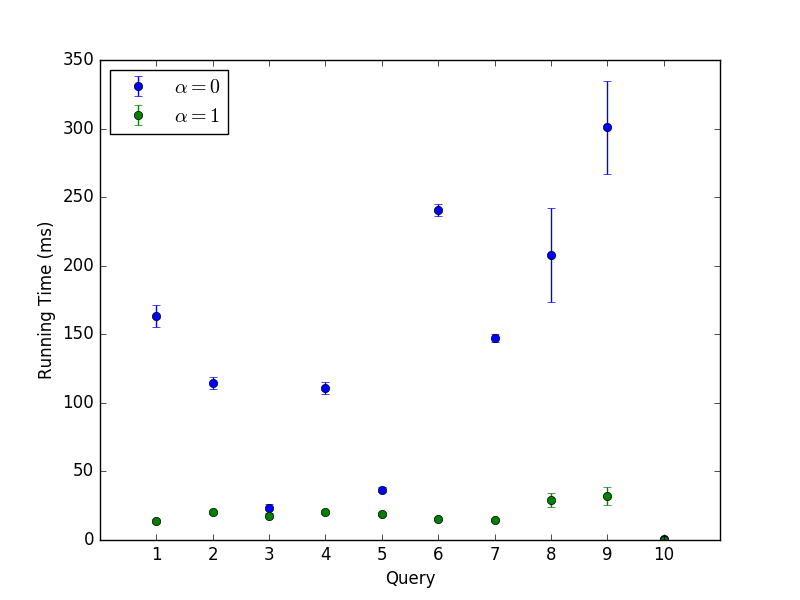
\includegraphics[width=\columnwidth]{figures/running_times_imputedb.png}
\caption{Query runtimes with \ProjectName{}}
\label{subfig:project-runtime-queries}
\end{subfigure}
~
\begin{subfigure}{\linewidth}
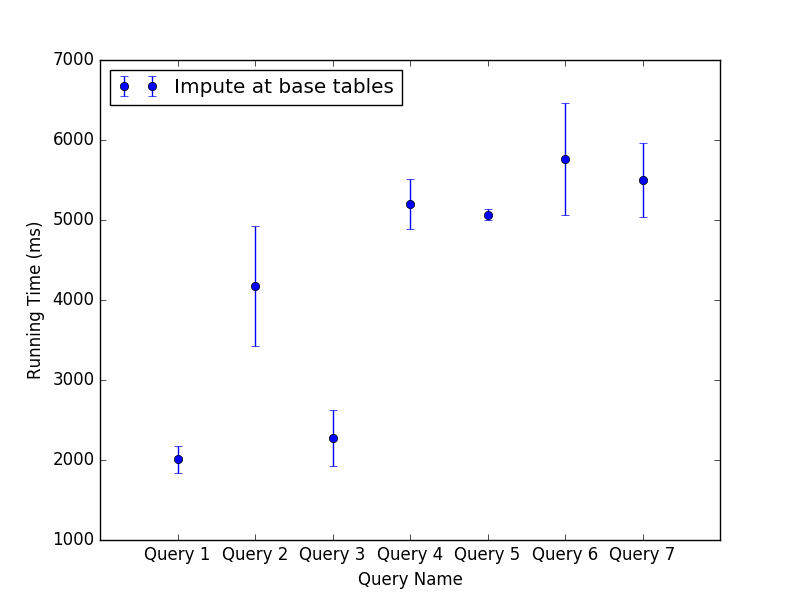
\includegraphics[width=\columnwidth]{figures/running_times_base_tables.png}
\caption{Query runtimes with imputation on base tables}
\label{subfig:base-runtime-queries}
\end{subfigure}
\caption{Comparing \ProjectName{} runtimes for each query (\ref{subfig:project-runtime-queries}) with the runtime for a query when base-table imputations are used (\ref{subfig:base-runtime-queries})}
\label{fig:runtimes}
\end{figure}

%TODO MJS
Figure~\ref{fig:plantimes} provides a summary of the planning times for each of the queries.  We exclude the planning time for queries that impute at base table, as that
requires no planning. On average, planning constituted 38 percent of total runtime for plans generated by \ProjectName{}.

\begin{figure}
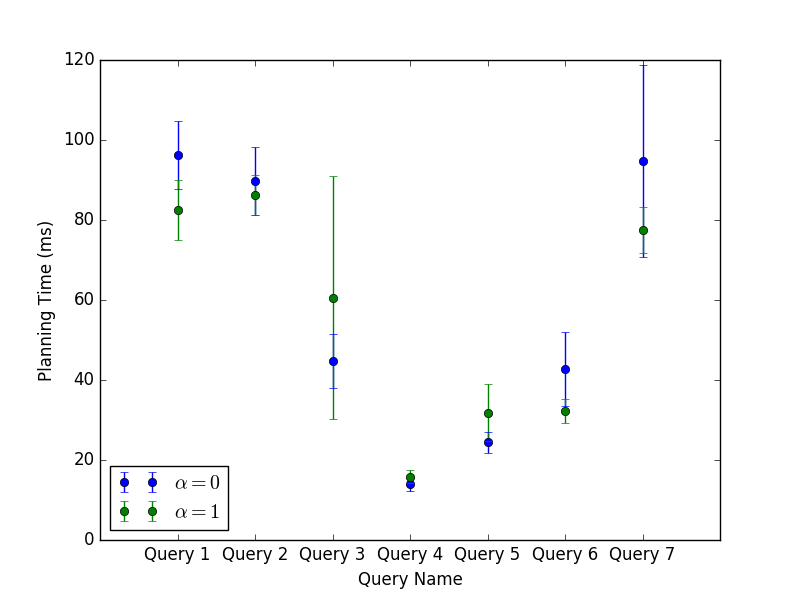
\includegraphics[width=\columnwidth]{figures/planning_times_imputedb.png}
\caption{Planning times for each query}
\label{fig:plantimes}
\end{figure}

Table~\ref{table:smape} shows the Symmetric-Mean-Absolute-Percentage-Error (SMAPE) for \ProjectName{}'s query results when compared to 
running imputation on the base tables and executing the query on the
cleaned data. Each query was run 10 %TODO MJS
iterations in both settings and then results from the two approaches were paired up and compared tuple-wise. We average tuple-wise
absolute percentage deviations within each iteration of a query, and we report this value averaged over all iterations.
We can see that optimizing for quality indeed reduces the SMAPE of query results. In general, the SMAPE relative to the
base-imputation approach are low in all cases, indicating that on-the-fly imputation produces similar results to
imputation at the base tables.

\begin{table}
\centering
\begin{tabular}{rrr}
\toprule
 Query &  \textbackslashalpha &  SMAPE \\
\midrule
     0 &     0.0 &   0.47 \\
     0 &     1.0 &   0.15 \\
     1 &     0.0 &   0.28 \\
     1 &     1.0 &   0.40 \\
     2 &     0.0 &   0.00 \\
     2 &     1.0 &   0.00 \\
     3 &     0.0 &   0.03 \\
     3 &     1.0 &   0.22 \\
     4 &     0.0 &  11.18 \\
     4 &     1.0 &    NaN \\
     5 &     0.0 &   0.79 \\
     5 &     1.0 &   1.93 \\
     6 &     0.0 &   0.00 \\
     6 &     1.0 &   0.03 \\
     7 &     0.0 &   0.82 \\
     7 &     1.0 &  35.44 \\
     8 &     0.0 &   0.23 \\
     8 &     1.0 &   0.31 \\
     9 &     0.0 & 100.00 \\
     9 &     1.0 & 100.00 \\
\bottomrule
\end{tabular}

\caption{Symmetric-Mean-Absolute-Percentage-Error for queries run under different $\alpha$ parameterizations relative to results when imputing on base table}
\label{table:smape}
\end{table}

% TODO MJS
In many cases, applying the imputation step at the base table simply is not an option. To illustrate the increasing difficulty of such an approach
as datasets scale, we used a simple aggregate query over the ACS dataset in our final experiment(Figure~\ref{query-acs}). Applying the imputation operation to the base table
is extremely expensive, in our case the process did not terminate within 20 minutes. In contrast, \ProjectName{} executes a quality-optimized version
in 9 seconds and a runtime-optimized version in 1 second. This highlights the potential benefit of using our system for early data exploration.

\begin{figure}
\begin{lstlisting}
SELECT AVG(c0) FROM acs_dirty;
\end{lstlisting}
\caption{A simple aggregate query on ACS data. Imputing the base table is undesirable (did not terminate within 20min). \ProjectName's
quality-optimized and performance-optimized query execute in 9 seconds and 1 second, respectively.
}%TODO MJS
\label{query-acs}
\end{figure}


%%% Local Variables:
%%% mode: latex
%%% TeX-master: "main"
%%% End:
